\documentclass[a4paper,parskip=half]{article} %scrartcl
\usepackage[utf8]{inputenc}
\usepackage[T1]{fontenc}
\usepackage{amsmath,mathtools,amssymb,listingsutf8,xspace}
\usepackage{geometry,hyperref,cleveref,xcolor}
\usepackage[disable]{todonotes}

\newcommand*\cmdstyle\texttt
\newcommand*\file\cmdstyle
\newcommand*\literalColor{blue}
\newcommand*\cmd[1]{\cmdstyle{\textcolor{red!85!black}{#1}}}
\newcommand*\cmdline[1]{\cmdstyle{\textcolor{green!70!black}\$ }\cmd{#1}}
\newcommand*\literal[1]{\textcolor{\literalColor}{\cmdstyle{#1}}}
\newcommand*\api[1]{\textcolor{purple}{\cmdstyle{#1}}}
\newenvironment{cmdhelp}{\begin{quote}\footnotesize}{\end{quote}}

\newcommand*\Solver{Symbolic Machine Learning Prover\xspace}
\newcommand*\SolverAbbrvText{SMLP}
\newcommand*\SolverAbbrv{\SolverAbbrvText\xspace}
\newcommand*\SolverVersion{v0.1}

\newcommand*\progmrc{smlp-mrc.sh}
\newcommand*\provenn{prove-nn.py}
\newcommand*\trainnn{train-nn.py}

\title{The \Solver}
\author{%
	Franz Brauße \and
	Zurab Khasidashvili \and
	Konstantin Korovin
}

\begin{document}
\maketitle
\begin{abstract}


\Solver (\SolverAbbrv) is a collection of tools for reasoning about machine
learning models. \SolverAbbrv is based on SMT solver(s). In this document we
desribe functionality for computing safe and stable regions of neural network
models satisfying optput specifications. This correponds to solving
$\epsilon$-guarded $\exists^*\forall^*$ formulas over NN
representations~\cite{BKK20}.

%\Solver (\SolverAbbrv) is a distribution of tools around an SMT-based solver for
%computing safety thresholds of functions defined by NNs on regions in bounded
%domains. At its core are the algorithms for solving $\epsilon$-guarded
%$\exists^*\forall^*$ formulas~\cite{BKK20}.

\SolverAbbrv has been developed by
\href{mailto:brausse@informatik.uni-trier.de?subject=\SolverAbbrvText}{Franz Brauße},
Zurab Khasidashvili
and Konstantin Korovin and is available
under the terms of the Apache License v2.0.%
\footnote{\url{https://www.apache.org/licenses/LICENSE-2.0}}
\end{abstract}
\tableofcontents

\section{Changes}
\begin{itemize}
\item 07/07/2020: documentation of \SolverAbbrv v0.1
\end{itemize}

%\section{Introduction}
\section{Concepts and Preliminaries}
In this document, syntactical highlights are placed on
\literal{literal strings}, which are ASCII sequences used to communicate input
to and output from programs; on \cmd{commands} to be executed;
and on \api{API references} which correspond to
either concrete symbols or abstract concepts defined in the corresponding API.

We assume familiarity with JSON, \cmd{make} and CSV files. Since the CSV format
is not unambiguously defined, we give the concrete requirements in
\cref{sec:csv}.

The glossary in this section defines concepts which are used throughout this
document when describing in detail the problems solved by \SolverAbbrv and is
meant to be referred to on an per-instance basis instead of reading it as a
whole.
\begin{description}
\item[Center Threshold]
	A rational value in $[0,1]$ larger or equal to Threshold.
\item[Codomain]
	A real vector space.
\item[Data set]
	A list of points in $D\times C$ where $D$ is the domain and $C$ is the
	codomain.
\item[Domain]
	A domain $D$ is the cartesian product $\bigtimes_{i=1}^n D_i$ where
	$D_i$ is a subset of either $\mathbb Z$, $\mathbb R$ or a
	discrete finite subset of $\mathbb Q$.
\item[Feature]
	Any column of a data set $\mathcal D$ is called a feature.
\item[Instance]
	A tuple
	$(N,\mathcal N_D,o,\mathcal N_o)$ is called an instance if
	$N$ is an NN over domain $D$, $\mathcal N_D$ is a data normalization,
	$o$ is an objective function and
	$\mathcal N_O$ is an objective normalization.
	If -- in addition to an instance $I$ -- a data set $\mathcal D$ over $D$
	is given, $(I,\mathcal D)$ is called a data instance.
\item[NN]
	Neural network as understood by the Keras API of Tensorflow in HDF5
	format.
	In particular, the \Solver only handles \api{Dense} layers with either
	\api{relu} or \api{linear} activation function.
	The input layer must be defined on domain $D$ and the output layer
	must map to the codomain $C$.
\item[Region]
	Given a domain $D=\bigtimes_{i=1}^d D_i$, a region (in $D$) is a
	product $\bigtimes_{i=1}^d C_i$ where
	each $C_i\subseteq D_i$ is a finite union of compact intervals for
	$i=1,\ldots,n$.
	For discrete $D_i$, e.g., a subset of $\mathbb Z$,
	$C_i$ is the finite union of point intervals.
	Otherwise, $D_i$ is a bounded subset of $\mathbb R$ and $C_i$
	corresponds to just one interval $[c_i\pm r_i]$ with center $c_i\in D_i$
	and rational radius $r_i>0$.
\item[Safe]
	A region $R$ is considered safe (wrt.\ a given target function $f$) for a
	constant $t\in\mathbb Q$ if $f$ satisfies $f(x)\geq t$
	for all $x\in R$.
\item[.spec]
	Specification file describing the domain, codomain and regions in the
	domain. Its format is a JSON list where the $i$-th entry corresponds to
	the $i$-th column in the CSV describing the data set.

	Given a data set and a .spec file, the components $D_i$ of the domain
	are defined as $D_i=E_i(F_i)$ where
	$E_i$ is called the embedding of $F_i$ into $D_i$ where $F_i$ is the
	$i$-th input feature.
%\item[Stable]
\item[Target function]
	The target function $f_I$ of an instance
	$I=(N,\mathcal N_D,o,\mathcal N_o)$ is defined as the composition
	$\mathcal N_o\circ o\circ\mathcal N_{D,\mathrm o}\circ
	N\circ\mathcal N_{D,\mathrm i}$.
	The target function $f_{I,\mathcal D}$ of a data instance
	$(I,\mathcal D)$ is
	$x\mapsto\min(\{f_I(x)\}\cup\{\mathcal N_o(o(y)):(x,y)\in\mathcal D\})$.
\item[Threshold]
	The threshold for a region $R$ and target function $f$ is defined
	as the maximal $t\in\{t_1,\ldots,t_n\}\subset[0,1]\cap\mathbb Q$ for
	which $R$ is safe wrt.\ $f$ for $t$ if it exists, and $-\infty$ otherwise.

	The threshold for a domain $D$ and target function $f$ is defined
	as the maximal $t\in\{t_1,\ldots,t_n\}\subset[0,1]\cap\mathbb Q$ for
	which there is a region that is safe wrt.\ $f$ for $t$ if it exists, and
	$-\infty$ otherwise.
\end{description}

%\section{Overview}



\section{Prerequisites}
This section describes software environments \SolverAbbrv is known to work in.
All packages corresponding to software listed in in \Cref{list:libs} should be
installed ``system-wide'',
meaning that they are accessible to the corresponding interpreter or compiler
listed in \Cref{list:comp-int} without additional options.

Please note, that \SolverAbbrv may run with versions of the packages not listed
here. These lists are subject to change and are gradually extended as soon as
more versions have been tested or other package requirements arise.

\subsection{Compilers / Interpreters / Utils}\label{list:comp-int}
These tools should be available in one of the paths
mentioned in the \texttt{PATH} environment variable.
\begin{itemize}
\item \cmd{bash}: GNU Bourne Again Shell version 5.0\_p17
	\url{http://tiswww.case.edu/php/chet/bash/bashtop.html}
\item \cmd{gmake}: GNU make version 4.1, 4.2 or 4.3
	\url{https://www.gnu.org/software/make/make.html}
\item \cmd{awk}: GNU awk version 5.0.1 or 5.1
	\url{https://www.gnu.org/software/gawk/gawk.html}
\item \cmd{sed}: GNU sed version 4.8
	\url{http://sed.sourceforge.net/}
\item GNU coreutils version 8.32
	\url{https://www.gnu.org/software/coreutils/}
\item GNU time version 1.7, 1.7.2 or 1.9
	\url{https://www.gnu.org/directory/time.html}
\item \cmd{cc}: either GNU C Compiler version 4.7.4, 5.4.0, 9.3.0 or 10.1.0
	\url{https://gcc.gnu.org/}
	or Clang version 10.0.0
	\url{https://clang.llvm.org/}
\item \cmd{python3}: CPython version 3.6 or 3.7
	\url{https://www.python.org/}
\end{itemize}

\subsection{Libraries}\label{list:libs}
The paths to the installed \texttt{python} directory should be set in the
\texttt{PYTHONPATH} environment variable. See \cmd{python3 -h} for details on
this variable.
\begin{itemize}
\item Tensorflow version 2.1 or 2.2 \url{https://www.tensorflow.org/}
\item Z3 including its Python API version 4.8.6 or 4.8.8
	\url{https://github.com/Z3Prover/z3}
\item Pandas version 0.24.2 \url{https://pandas.pydata.org/}
\item scikit-learn version 0.20.4 or 0.22.2\_p1
	\url{https://scikit-learn.org/}
\item matplotlib version 2.2.4 or 3.1.2
	\url{https://matplotlib.org/}
\item seaborn version 0.9.x or 0.10.x
	\url{https://seaborn.pydata.org/}
\item HDF5 for Python version 2.10.0
	\url{https://www.h5py.org/}
\item kjson version 0.1.3 (bundled in release)
	\url{https://github.com/fbrausse/kjson}
\end{itemize}


\section{Training ML models with SMLP}\label{sec:models}

SMLP supports training tree-based and polynomial models using the scikit-learn\footnote{\url{https://scikit-learn.org/stable/}} and pycaret\footnote{\url{https://pycaret.org}} packages, 
and training neural networks using the Keras package with TensorFlow\footnote{\url{https://keras.io}}. For systems with multiple outputs, SMLP supports training one model with multiple outputs as well as training separate models per response (this is controlled by command-line option $model\_per\_response$). Supporting these two options allows a trade-off between the accuracy of the models (models trained per response are likely to be more accurate) and with the size of the formulas that represent the model for symbolic analysis (one multi-output model formula will be at least smaller when the same training hyper-parameters are used). Conversion of models to formulas into SMLP language is done internally in SMLP (no encoding options are exposed to user in current implementation, which will change once alternative encodings will be developed).



\section{ML model exploration with SMLP}\label{sec:exploration}

SMLP supports the following model exploration modes (we assume that an ML model $M$ has already been trained). A formal definition of the tasks accomplished with these model exploration modes can be found in~\cite{BKK24}.

\begin{itemize}
\item[certify] Given an ML model $M$, a value assignment $a$ to knobs, and a query $q$, check that $a$ is a stable witness for query $q$ on model $m$. Multiple pairs $(a,q)$ of candidate witness $a$ and query $q$ can be checked in a single SMLP run.
\item[query] Given an ML model $M$  and a query $q$, find a stable witness $a$  for query $q$ on model $M$.
\item[verify] Given an ML model $M$,  a value assignment $a$ to knobs,  and an assertion $assert$, verify whether the assertion is valid on model $M$ for any legal inputs (for the given value assignment $a$ to knobs). SMLP supports verifying multiple assertions in a single run.
\item[synthesize] Given an ML model $M$,  find a stable configuration of knobs (a value assignment $a$ to knobs) such that required constraints (possibly including assertions),  are valid for all legal value assignments to the inputs.
\item[optimize]  Given an ML model $M$,  find a stable configuration of knobs that yields a pareto-optimal values of the optimization objectives (pareto-optimal with respect to the \emph{max-min} optimization problem defined in~\cite{BKK24}.
\item[optsyn] Given an ML model $M$,  find a stable configuration of knobs that yields a pareto-optimal values of the optimization objectives and all constraints and assertions are valid for all legal values of inputs. This mode is a union of the \emph{optimize} and \emph{synthesize} modes, its full name is \emph{optimized synthesis}. All the previous modes can be seen as a special case of optimized synthesis mode.
\end{itemize}


\section{How to run SMLP}\label{sec:mrc}


Consider a toy dataset in Table~\cref{toy_basic_df} with two inputs $x_1, x_2$, two knobs $i_1, i_2$, and two outputs $y_1, y_2$.
Command to run SMLP in \emph{optimize} mode is given in Figure~\cref{fig:command}.
The optimization problem is specified in the spec file in Figure~\cref{fig:spec}.

\begin{table*}[t]
\centering\small
\begin{tabular}{lrrrrrr}
\hline %\toprule
{} &      x1 &  x2 &    p1 &  p2 &       y1 &       y2 \\
\hline %\midrule
0 &  2.9800 &  -1 &   0.1 &   4 &   5.0233 &   8.0000 \\
1 &  8.5530 &  -1 &   3.9 &   3 &   0.6936 &  12.0200 \\
2 &  0.5580 &   1 &   2.0 &   4 &   0.6882 &   8.1400 \\
3 &  3.8670 &   0 &   1.1 &   3 &   0.2400 &   8.0000 \\
4 & -0.8218 &   0 &   4.0 &   3 &   0.3240 &   8.0000 \\
5 &  5.2520 &   0 &   4.0 &   5 &   6.0300 &   8.0000 \\
6 &  0.2998 &   1 &   7.1 &   6 &   0.9100 &  10.1250 \\
7 &  7.1750 &   1 &   7.0 &   7 &   0.9600 &   1.1200 \\
8 &  9.5460 &   0 &   7.0 &   6 &  10.7007 &   9.5661 \\
9 & -0.4540 &   1 &  10.0 &   7 &   8.7932 &   6.4015 \\
\hline %\bottomrule
\end{tabular}
\caption{Toy dataset with two inputs $x_1, x_2$, two knobs $i_1, i_2$, and two outputs $y_1, y_2$.}
\label{toy_basic_df}
\end{table*}

\begin{figure}%[tp]
%\scriptsize
%\tiny
%\small
\begin{verbatim}
 ../src/run_smlp.py -data smlp_toy_basic -out_dir out -pref abc  -mode optimize -pareto t  \
-sat_thresh f -resp y1,y2 -feat x1,x2,p1,p2 -model dt_sklearn -dt_sklearn_max_depth 15 \
-data_scaler min_max -epsilon 0.05 -delta 0.01 -save_model_config f -mrmr_pred 0 -plots f \
-seed 10 -log_time f -spec smlp_toy_basic
\end{verbatim}
\caption{Example of SMLP's command to build a decision tree model and find .}
\label{fig:command}
\end{figure}



\begin{figure}%[tp]
%\scriptsize
%\tiny
\small
\begin{verbatim}
{
  "version": "1.2",
  "variables": [
    {"label":"y1", "interface":"output", "type":"real"},
    {"label":"y2", "interface":"output", "type":"real"},
    {"label":"x1", "interface":"input", "type":"real", "range":[0,10]},
    {"label":"x2", "interface":"input", "type":"int", "range":[-1,1]},
    {"label":"p1", "interface":"knob", "type":"real", "range":[0,10], "rad-rel":0.1, "grid":[2,4,7]},
    {"label":"p2", "interface":"knob", "type":"int", "range":[3,7], "rad-abs":0.2}
  ],
  "alpha": "p2<5 and x1==10 and x2<12",
  "beta": "y1>=4 and y2>=8",
  "eta": "p1==4 or (p1==8 and p2 > 3)",
  "assertions": {
    "assert1": "(y2**3+p2)/2>6",
    "assert2": "y1>=0",
    "assert3": "y2>0"
  },
  "objectives": {
    "objective1": "(y1+y2)/2",
    "objective2": "y1"
  }
}
\end{verbatim}
\begin{tikzpicture}[remember picture,overlay,shift={(22em,\baselineskip)}]
\node[anchor=south west]{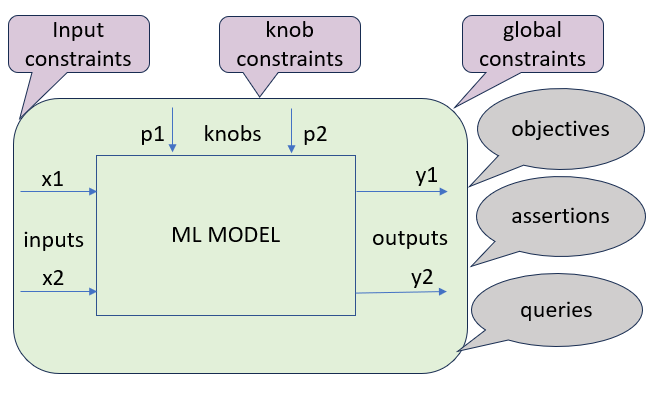
\includegraphics[height=14\baselineskip]{smlp_encoding.PNG}};
\end{tikzpicture}
\vspace*{-1\baselineskip}
\caption{Specification $smlp\_toy\_basic$ used by SMLP command in Figure~\cref{fig:command}.}
\label{fig:spec}
\end{figure}







\section{MRC usage}\label{sec:mrc}

Quick command template for solving the MRC problem on a single machine:
\begin{equation}
\cmdline{\progmrc{} -i \emph{data.csv} -s \emph{data.spec} -t \emph{target/dir} -j 112 run}
\tag{$*$}\label{cmd:mrc}
\end{equation}
Here, \file{\emph{data.csv}} is the data set containing training samples,
\file{\emph{data.spec}} is the specification file detailed in \cref{sec:.spec}\todo{add example in release or documentation},
\cmdstyle{-t \emph{target/dir}} is an optional working directory for the prover and \cmdstyle{-j 112} is the maximum number of parallel jobs to run.

For each combination of categorical parameters \literal{CH} and \literal{Byte}s the tool: 
\begin{enumerate}
\item builds a NN model representing the target function,
\item computes thresholds and safe and stable regions for these representation,
\item extends regions and thresholds to other bytes in the channel.
\end{enumerate}

The output will be a file \file{\emph{target/dir}/rank0/shared1.csv} containing
the safe and stable regions and thresholds across all \literal{Byte}s for each
\literal{CH}.
%, see also \cref{sec:mrc-def}.
\todo{output format/values/meaning}

For details, please see the following sections.


\subsection{Problem definition}\label{sec:mrc-def}
Assume a data set containing, besides other integer or floating-point features,
the categorical input features \literal{Byte},
\literal{CH} and \literal{RANK} ranging over
$\{\literal0,\literal1,\literal2,\literal3,\literal4,\literal5,\literal6,\literal7\}$,
$\{\literal0,\literal1\}$ and $\{\literal0\}$, respectively,
is described in the CSV file \file{data.csv}. Furthermore, assume the codomain
is labelled \literal{delta}.

The goal is to find, for each \literal{Byte} and \literal{CH},
\begin{enumerate}
\def\labelenumi{(\alph{enumi})}
\item a threshold $t$ among $\{0.05\cdot i:i=0,\ldots,20\}$ for which safe
	regions exist,
\item $n\leq 100$ safe regions $R_1,R_2,\ldots,R_n$, which satisfy the .spec and
\item thresholds for all $R_i$ among $\{0.05\cdot i:i=0,\ldots,20\}$ for the
	other \literal{Byte}s in this \literal{CH}.
\end{enumerate}
The data instances $(I^{c,b},\mathcal D^{c,b})$ with
$I^{c,b}=(N^{c,b},\mathcal N_D^{c,b},o,\mathcal N_o^c)$
defining the target function $f_{I^{c,b},\mathcal D^{c,b}}$ for which the
above thresholds should hold is defined for each \literal{CH}/\literal{Byte}
combination $(c,b)$ by
\begin{itemize}
\item the .spec file \file{data.spec} defining the domain $D$
	and the finite set of regions, see \cref{sec:.spec}, and
\item the data set
	%$\bigcup_{c\in\{0,1\}}\bigcup_{b\in\{0,\ldots,7\}}\mathcal D^{c,b}$
	described by the CSV file \file{data.csv}, where
	the restriction and projection to $(c,b)$, $\mathcal D^{c,b}$,
	is a subset of the domain $D$
\end{itemize}
in the following way:
\begin{itemize}
\item
	The NN $N^{c,b}$ is defined by the training algorithm on
	$\mathcal D^{c,b}$.
\item
	The data normalization $\mathcal N_D^{c,b}$ corresponds to the pair of
	normalization $N_{D,\mathrm i}^{c,b}=\operatorname{norm}_{I^{c,b}}$
	and denormalization
	$N_{D,\mathrm o}^{c,b}=\operatorname{norm}_{J^{c,b}}^{-1}$ where
	$\operatorname{norm}_{[\vec a,\vec b]}:\vec x\mapsto ((x_i-a_i)/(b_i-a_i))_i$
	is the component-wise normalization to domain bounds $I^{c,b}$
	defined by $\mathcal D^{c,b}$
	and $\operatorname{norm}_{J^{c,b}}^{-1}$ is the inverse of
	$\operatorname{norm}_{J^{c,b}}$
	where $J^{c,b}$ are the codomain bounds defined by $\mathcal D^{c,b}$.

	This definition assumes $I^{c,b}$ and $J^{c,b}$ do not contain
	point intervals.
\item
	Objective funtion $o$ is the projection to the first component
	\literal{delta} (i.e.\ the identity).
\item
	The objective normalization $\mathcal N_o^c=\operatorname{norm}_{C_c}$
	is shared across all $b$ per $c$ and defined on the bounds $C_c$ of the
	objective function $o$ on $\bigcup_{b\in\{0,\ldots,7\}}\mathcal D_{c,b}$
	projected to the codomain.
\end{itemize}

By the above definition, the entries besides
\literal{"obj-bounds"} and \literal{"train"}
in the derived instance description file
\file{\emph{target/dir}/rank0/ch\{0,1\}/byte/\{0..7\}/model\_gen\_*\_12.json}
(see \cref{sec:.gen} for details) are fixed.
It should have the following form:
\begin{quote}\footnotesize\color{\literalColor}\begin{verbatim}
{
   "obj-bounds" : {
      "max" : 68,
      "min" : -57.6
   },
   "objective" : "delta",
   "pp" : {
      "features" : "min-max",
      "response" : "min-max"
   },
   "response" : [
      "delta"
   ],
   "train" : {
      "activation" : "relu",
      "batch-size" : 32,
      "epochs" : 30,
      "optimizer" : "adam",
      "seed" : 1234,
      "split-test" : 0.2
   }
}
\end{verbatim}\end{quote}


\subsection{How to use \SolverAbbrv to solve the MRC problem}

The following steps are performed during the run of \SolverAbbrv on the MRC
problem when the command \eqref{cmd:mrc}  given at the beginning of
\cref{sec:mrc}, is invoked. We assume that the user provided a specification
file \file{data.spec} and training data set in the file \file{data.csv}.
Although the system does not require futher interaction we give commands that
can be performed to execute the corresponding steps separately  (and its
dependencies) here as well.

%problem for the version of \Solver described here.
%The following steps are required to solve the MRC problem for the version of
%\Solver described here.
%Though steps corresponding to \cref{step:shai:2,step:shai:3,step:shai:4,step:shai:5} can
%be performed automatically by invoking
%the command \eqref{cmd:mrc} given at the beginning of \cref{sec:mrc},
%we also give the concrete commands to just perform the
%corresponding step (and its dependencies) here as well.
\begin{enumerate}
%\item\label{step:shai:1}
%	Write a specification file \file{data.spec}.
\item\label{step:shai:2}
	Split the data set into $2\cdot8$ data sets and set up the corresponding
	subdirectories \file{rank0/ch$c$/byte/$b$/} for the next steps,
	one for each combination $(c,b)$ of \literal{CH} and \literal{Byte}.

	\cmdline{\progmrc{} -i \emph{data.csv} -s \emph{data.spec}
		-t \emph{target/dir}
		run prepare}

	resulting in a directory tree at \emph{\file{target/dir}} prepared for
	the following steps.
\item\label{step:shai:3}
	Train NNs for all $(c,b)$.

	In \file{\emph{target/dir}}: \cmdline{\progmrc{} -j 16 run train}
\item\label{step:shai:4}
	Find thresholds and safe regions for each $(c,b)$.

	In \file{\emph{target/dir}}: \cmdline{\progmrc{} -j 16 run search}
\item\label{step:shai:5}
	For each $c$, determine thresholds of $R$ for $(c,b')$
	for each $R,b,b'$ where $b'\neq b$ and $R$ has been found safe for
	$(c,b)$ in \cref{step:shai:4} and
%\item
	collect results into \file{shared1.csv}.

	In \file{\emph{target/dir}}: \cmdline{\progmrc{} -j 112 run collect}
\end{enumerate}
Each of these steps depends on the previous.
%The only step to be performed manually is \cref{step:shai:1}.
The parameter \cmdstyle{-j \emph N} in the above commands is optional and
denotes the maximum number of parallel jobs to use. The values \cmdstyle{\emph N}
given above are the maximum bounds on the number of parallel jobs that
-- given enough resources -- may provide a noticable speedup of the entire
computation.


\subsection{Internals and control files for the MRC instance}
In order to change defaults for various settings, we briefly describe the
important configuration files as set up by the \cmdstyle{prepare} stage of
\cmd{\progmrc} and how the solver invocations for multiple \literal{CH} and
\literal{Byte} combinations are performed.

The parallel execution of the steps in
\cref{step:shai:3,step:shai:4,step:shai:5} of the previous section
is delegated to \cmd{make} by means of the
following \file{Makefile}s generated by \cref{step:shai:2} in
\emph{\file{target/dir}}:
\begin{enumerate}
\item\label{mk:rank} \file{rank0/Makefile}

	Entry point; delegation to \cref{mk:byte} for \cmd{make} targets
	\cmdstyle{train} and \cmdstyle{search}.
	Delegates to \cref{mk:ch} for the \cmdstyle{collect} target and
	generates the result file \file{rank0/shared1.csv}.

\item\label{mk:ch} \file{rank0/ch\{0,1\}/Makefile}

	Delegates \cref{mk:byte} for the \cmdstyle{collect} target,
	synchronizes the computations of the shared safe regions and
	collects the results in \file{rank0/ch\{0,1\}/shared1.csv}.

\item\label{mk:byte} \file{rank0/ch\{0,1\}/byte/\{0..7\}/Makefile}

	Main driver: Runs the search for a specific $(c,b)$ combination either
	with (for the \cmdstyle{collect} target in \cref{mk:rank}) or without
	(for the \cmdstyle{search} target in \cref{mk:rank}) by taking into
	account customizations defined in the \file{params.mk} files in the
	following paths under \emph{\file{target/dir}} as well as
	\file{src/defaults.mk} and \file{src/scripts.mk}.
	Each \file{params.mk} above one in a subdirectory gives defaults for
	the latter.

	\begin{itemize}
	\item\file{params.mk}
	\item\file{rank0/params.mk}
	\item\file{rank0/ch\{0,1\}/params.mk}
	\item\file{rank0/ch\{0,1\}/byte/\{0..7\}/params.mk}
	\end{itemize}

	As generated by the \cmdstyle{prepare} stage of \cmd{\progmrc},
	all but the top-level \file{params.mk} just delegate to the one
	immediately above. The top-level one maintains defaults for the MRC
	application, such as defining $N_o$ and the specific \cmd{make} targets
	for computing shared regions across one \literal{CH}.

	The template used by the \cmdstyle{prepare} stage for the top-level file
	can be found in \file{src/mrc-params.mk} while the remaining ones are
	generated. %by \cmd{src/split-categorical2.py} which is called indirectly.

	\file{rank0/ch\{0,1\}/byte/\{0..7\}/Makefile} is a symlink to the
	template \file{src/datasets.mk} distributed with \SolverAbbrv and
	created in the \cmdstyle{prepare} stage.
\end{enumerate}


\subsection{MRC options}
\begin{cmdhelp}\begin{verbatim}
smlp-mrc.sh [-OPTS] COMMAND [ARGS...]

Common options [defaults]:
  -d           debug this script
  -h           print this help message
  -k           keep created files / directories on errors
  -j JOBS      run N jobs in parallel; if JOBS is 0 determine via lscpu(1) [1]
  -t TGT       path to target instance directory [derived from basename of SRC
               if given, otherwise '.']

Options used by 'prepare' stage:
  -i SRC       path to source data set ending in .csv
  -s SPEC      path to .spec file describing the target instance

Options used by 'train' stage [defaults replicated from src/defaults.mk]:
  -b BATCH     batch size [32]
  -e EPOCHS    number of epochs to use for training [30]
  -f FILTER    percentile of lowest OBJT values to ignore for training [0]
  -l LAYERS    layer specification [2,1]
  -o OBJT      objective function [RESP]
  -r RESP      response features [delta]
  -s SEED      random number seed for numpy and tensorflow [1234]

Options used by 'search' and 'collect' stages
[defaults replicated from src/defaults.mk]:
  -c COFF      center threshold offset from threshold [0.05]
  -n N         restrict to maximum of N safe regions [100]
  -L TLO       minimum threshold to consider [0.00]
  -H THI       maximum threshold to consider [0.90]

Commands [defaults]:
  run [STAGE]  execute all stages up to STAGE [collect]

Stages (in dependency order):
  prepare      use SRC to setup a fresh TGT instance
  train        train NN models according to prepared TGT instance
  search       determine safety thresholds for TGT instance
  collect      collect shared safe regions
\end{verbatim}\end{cmdhelp}





\section{Components}

%Due to the current version of \Solver being the result of general research into
%the problem, automation has not been the priority.
This section provides an
overview of the individual components involved in the use cases described in
\cref{sec:mrc}, gives an overview of the full functionality as implemented
in the current version and provides details about the .spec file and
the derived instance description.

\subsection{Introduction}
The tools distributed in \SolverAbbrv can be used stand-alone to solve a
specific problem. However, in order to find thresholds for the existence of safe
regions, that is, solving the discretized optimization problem
\[ \max\{t\in\{t_1,\ldots,t_n\}\mid \exists R.\,R~\text{is safe wrt.}~t\} \]
in addition to determining
\[ t_{R,I}=\max\{t\in\{t_1,\ldots,t_n\}\mid R~\text{is safe wrt.}~t~\text{in}~I\} \]
for given regions $R$ and multiple instances $I$,
the wrapper script \cmd{\progmrc} along with default \cmd{make} template
files specifically tailored for the MRC problem are included.
The MRC problem is defined in detail in \cref{sec:mrc}.

The core solver is \cmd{src/\provenn}. It has many options regarding
specific search strategies, domain grids, bounds modifying the target function
as well as other heuristics. Details can be found in \cref{sec:nn_model2.py}.

The program \cmd{src/\trainnn} takes care of training NNs on data
sets and writing information about domain- and codomain-normalization, the
correspondence between NN output(s) and the data set's features as well as
the objective function and bounds into the files \file{data\_bounds\_*\_12.json}
(containing only the features' bounds) and \file{model\_gen\_*\_12.json}
(containing the remaining parameters, called derived instance description).

The version of \SolverAbbrv described here is referred to as \SolverVersion.


\subsection{Specification file}\label{sec:.spec}
Specification file contains description of the domain of the target function, which  can also include domain grid. 

%All tools operating on the grid or domain require at least a specification
%(.spec file), usually called \file{data.spec}.
It is used to define the domain of the target function, the radii of the
regions under consideration and the quantification over the domain.

The specification file format and its correspondence to domain and regions is
described in \file{doc/spec.pdf} and subject to change.


\subsection{Derived instance description}\label{sec:.gen}
The derived instance description file usually called
\file{model\_gen\_data\_12.json} contains a JSON object with at least
the following entries. It can be generated by
\cmd{src/\trainnn}.
\begin{description}
\item[\literal{"obj-bounds"}:]
	Numeric entries in a sub-object under keys \literal{"min"} and
	\literal{"max"} defining the bounds on the objective function on the
	data set used for training.
\item[\literal{"objective"}:]
	A string of one of the following patterns describing the form of the
	objective function to be applied to the output of the NN.
	\begin{itemize}
	\item\literal{"\emph{feature}"}:
		projection to \literal{\emph{feature}}, e.g. \literal{"delta"}.
	\item\literal{"\emph{feature$_1$}-\emph{feature$_2$}"}:
		projection to \literal{\emph{feature$_1$}} minus the
		projection to \literal{\emph{feature$_2$}}; e.g.
		\literal{"Up-Down"}.
	\end{itemize}
\item[\literal{"pp"}:]
	Sub-object containing information about data normalization
	(pre-/postprocessing) for values in the domain (\literal{"features"})
	and codomain (\literal{"response"}), each taking either the string
	\literal{"min-max"} for normalization based on bounds in the file
	\file{data\_bounds\_*\_12.json} or \literal{null} for no normalization.
\item[\literal{"response"}:]
	An ordered list containing the feature labels corresponding to
	\literal{"type": "response"} objects in the .spec file.
\end{description}
The object may optionally contain parameters used for training the NN model under
the key \literal{"train"}.


\subsection{Training NNs}
Performed by \cmd{src/\trainnn}, which has the following options:
\begin{cmdhelp}\begin{verbatim}
usage: src/train-nn.py [-h] [-a ACT] [-b BATCH] [-B BOUNDS] [-c [CHKPT]]
                       [-e EPOCHS] [-f FILTER] [-l LAYERS] [-o OPT]
                       [-O OBJECTIVE] [-p PP] [-r RESPONSE] [-R SEED] -s SPEC
                       [-S SPLIT]
                       DATA

positional arguments:
  DATA                  Path excluding the .csv suffix to input data file
                        containing labels

optional arguments:
  -h, --help            show this help message and exit
  -a ACT, --nn_activation ACT
                        activation for NN [default: relu]
  -b BATCH, --nn_batch_size BATCH
                        batch_size for NN [default: 200]
  -B BOUNDS, --bounds BOUNDS
                        Path to pre-computed bounds.csv
  -c [CHKPT], --chkpt [CHKPT]
                        save model checkpoints after each epoch; optionally
                        use CHKPT as path, can contain named formatting
                        options "{ID:FMT}" where ID is one of: 'epoch', 'acc',
                        'loss', 'val_loss'; if these are missing only the best
                        model will be saved [default: no, otherwise if CHKPT
                        is missing: model_checkpoint_DATA.h5]
  -e EPOCHS, --nn_epochs EPOCHS
                        epochs for NN [default: 2000]
  -f FILTER, --filter FILTER
                        filter data set to rows satisfying RESPONSE >=
                        quantile(FILTER) [default: no]
  -l LAYERS, --nn_layers LAYERS
                        specify number and sizes of the hidden layers of the
                        NN as non-empty colon-separated list of positive
                        fractions in the number of input features in, e.g.
                        "1:0.5:0.25" means 3 layers: first of input size,
                        second of half input size, third of quarter input
                        size; [default: 1 (one hidden layer of size exactly
                        #input-features)]
  -o OPT, --nn_optimizer OPT
                        optimizer for NN [default: adam]
  -O OBJECTIVE, --objective OBJECTIVE
                        Objective function in terms of labelled outputs
                        [default: RESPONSE if it is a single variable]
  -p PP, --preprocess PP
                        preprocess data using "std, "min-max", "max-abs" or
                        "none" scalers. PP can optionally contain a prefix
                        "F=" where F denotes a feature of the input data by
                        column index (0-based) or by column header. If the
                        prefix is absent, the selected scaler will be applied
                        to all features. This parameter can be given multiple
                        times. [default: min-max]
  -r RESPONSE, --response RESPONSE
                        comma-separated names of the response variables
                        [default: taken from SPEC, where "type" is "response"]
  -R SEED, --seed SEED  Initial random seed
  -s SPEC, --spec SPEC  .spec file
  -S SPLIT, --split-test SPLIT
                        Fraction in (0,1) of data samples to split from
                        training data for testing [default: 0.2]
\end{verbatim}\end{cmdhelp}

\subsection{General safety thresholds}\label{sec:nn_model2.py}
Performed by \cmd{src/\provenn} optionally with the help of
\cmd{src/libcheck-data.so}, which has these options:
\begin{cmdhelp}\begin{verbatim}
usage: src/prove-nn.py [-h] [-b [BOUNDS]] [-B DBOUNDS] [-C CHECK_SAFE]
                       [-d DATA] -g MODEL_GEN [-G GRID] [-n N] [-N]
                       [-o OUTPUT] [-O OBJECTIVE] [-r RESPONSE_BOUNDS] -s SPEC
                       [-S SAFE] [-t THRESHOLD] [-T SAFE_THRESHOLD]
                       [-U CENTER_OFFSET] [-v] [-x TRACE] [-X]
                       NN_MODEL

positional arguments:
  NN_MODEL              Path to NN model in .h5 format

optional arguments:
  -h, --help            show this help message and exit
  -b [BOUNDS], --bounds [BOUNDS]
                        bound variables [default: none; otherwise, if BOUNDS
                        is missing, 0]
  -B DBOUNDS, --data-bounds DBOUNDS
                        path to data_bounds file to amend the bounds
                        determined from SPEC
  -C CHECK_SAFE, --check-safe CHECK_SAFE
                        Number of random samples to check for each SAFE config
                        found [default: 1000]
  -d DATA, --data DATA  path to DATA.csv; check DATA for counter-examples to
                        found regions
  -g MODEL_GEN, --model-gen MODEL_GEN
                        the model_gen*.json file containing the training /
                        preprocessing parameters
  -G GRID, --grid GRID  Path to grid.istar file
  -n N                  number of safe regions to generate in total (that is,
                        including those already in SAFE) [default: 1]
  -N, --no-exists       only check GRID, no solving of existential part
  -o OUTPUT, --output OUTPUT
                        Path to output .smt2 instance [default: none]
  -O OBJECTIVE, --objective OBJECTIVE
                        Objective function in terms of labelled outputs
                        [default: "delta"]
  -r RESPONSE_BOUNDS, --response-bounds RESPONSE_BOUNDS
                        Path to bounds.csv for response bounds to interpret T
                        and ST in [default: use DATA_BOUNDS]
  -s SPEC, --spec SPEC  Path to JSON spec of input features
  -S SAFE, --safe SAFE  Path to output found safe configurations to as CSV
  -t THRESHOLD, --threshold THRESHOLD
                        Threshold to restrict output feature to be larger-
                        equal than [default: search in 0.05 grid between 0 and
                        0.95]
  -T SAFE_THRESHOLD, --safe_threshold SAFE_THRESHOLD
                        Center threshold [default: THRESHOLD+SAFE_OFFSET].
                        Overrides any SAFE_OFFSET.
  -U CENTER_OFFSET, --center_offset CENTER_OFFSET
                        Center threshold offset of threshold [default: 0]
  -v, --verbose         Increase verbosity
  -x TRACE, --trace-exclude TRACE
                        exclude all unsafe i* from trace file
  -X, --trace-exclude-safe
                        exclude also found safe i* from the trace file
\end{verbatim}\end{cmdhelp}


\subsection{Safety thresholds for concrete regions}
Performed by \cmd{src/\provenn} optionally with the help of
\cmd{src/libcheck-data.so}, by passing parameters
\cmdstyle{-NG \emph{path/to/safe/regions.csv}} set via
\begin{quote}
	\file{\emph{target/dir}/rank0/ch\{0,1\}/byte/\{0..7\}/lock.mk}
\end{quote}
which is generated at the end of the \cmdstyle{search} stage.

\subsection{Helper modules}
\subsubsection{\file{libcheck-data.so}}
C-library with Python wrapper defined in \file{checkdata.py} allowing to find
points in the data set within regions defined in the .spec file fast.

\subsubsection{\cmd{split-categorical2.py}}
Helper script for preparing the directory structure according to the MRC
application.

\subsubsection{\cmd{filter-trace.sh}}
Shell script for processing trace files into a more human-readable format by
filtering out non-SMT-related steps and displaying rational solutions as
decimal float approximations.



\begin{thebibliography}{99}
\bibitem{BKK20}
 F. Brauße, Z. Khasidashvili and K. Korovin.
\newblock{Selecting Stable Safe Configurations for Systems Modelled by Neural Networks with ReLU Activation.}
\newblock{2020 Formal Methods in Computer Aided Design, FMCAD 2020}
\newblock{IEEE, 2020}.

\bibitem{BKK22}
 F. Brauße, Z. Khasidashvili and K. Korovin.
\newblock{Combining Constraint Solving and Bayesian Techniques for System Optimization.}  
\newblock{31st International Joint Conference on Artificial Intelligence and the 25th European Conference on Artificial Intelligence, IJCAI-ECAI'22 2022.}


\bibitem{BKK24}
 F. Brauße, Z. Khasidashvili and K. Korovin.
\newblock{SMLP: Symbolic Machine Learning Prover.}
\newblock{Report arXiv: 2402.01415 , 2024.}
\end{thebibliography}


\appendix
\section{Concrete Formats}
\subsection{CSV}\label{sec:csv}
A structured line-based text format where the first line describes a
list of column headers and each line after it describes a list the
values corresponding to the respective column in the data set.
A line describes a list of elements $(e_i)_{i=1}^n$, if it corresponds
to the concatenation
$s(e_1)\literal,s(e_2)\literal,\ldots\literal,s(e_n)$
where $s(v)$ is the ASCII representation of $v$.

The list of column headers shall not contain duplicates.
The ASCII representation of ASCII strings made up of printable
characters excluding ``\literal,'' is the identity.
Floating point approximations are represented as the decimal encoding
where ``\literal.'' is the separator between integer and fractional
part. Rational numbers $\frac pq$ are represented by $s(p)\literal/s(q)$
where $s(z)$ is the decimal encoding of $|z|$ prefixed by ``\literal-''
if $z\in\mathbb Z$ is negative.



\end{document}
